\section{Marco Teórico} 



\subsection{Modelo Dimensional}
El modelado dimensional es una técnica de diseño lógico que busca presentar la información en un marco estándar e intuitivo que permita un acceso de alto rendimiento. Este modelado se vale de los principios de la disciplina que emplea el modelo relacional con algunas importantes restricciones. El modelado dimensional es esencialmente útil para resumir y organizar los datos y la presentación de información para soportar el análisis de la misma. Existen algunos conceptos básicos para comprender la filosofía de este tipo de modelado: áreas temas, medidas, dimensiones y hechos. \newline


Un área tema como es una cuestión de interés de una función empresarial. Las áreas tema en conjunto constituyen el ámbito de implementación del Data Warehouse. Por ejemplo, el departamento de Comercialización de una empresa puede estar interesado en las áreas tema de Pedidos, Promociones, Mercados y Ventas.  \newline


Para especificar las áreas tema se deben identificar las medidas. Una medida o indicador es un cuantificador del desempeño de un ítem o una actividad del negocio. La información que brinda una medida es usada por los usuarios en sus consultas para evaluar el desempeño de un área tema. Ejemplos de medidas son duración de las llamadas y cantidad de llamadas.  \newline

El Data Warehouse organiza un gran conjunto de datos operacionales mediante múltiples dimensiones. Una dimensión es una colección de miembros o entidades del mismo tipo y constituye un calificador conceptual que provee el contexto o significado para una medida. Ejemplos de dimensiones son Tipo de Llamada, Tiempo, Líneas y Organización Telefónica (Áreas e Internos). \newline

La forma de representar la organización de los datos en un modelo dimensional es a través de un cubo (el cual no necesariamente debe tener tres dimensiones). Por ejemplo, podemos pensar en un cubo que posea como medida Duración de las Llamadas y como dimensiones Tiempo, Tipo de Llamada y Organización Telefónica. \newline

\begin{center}
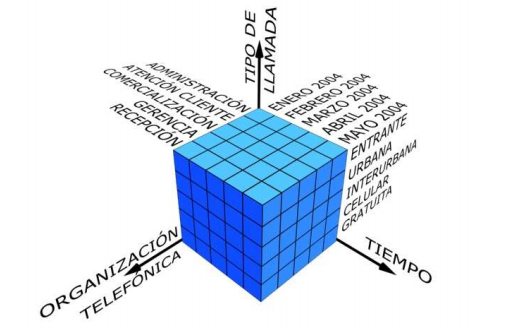
\includegraphics{images/BS/imagen 01.png}\newline
\end{center}




Cada porción del cubo de la Figura 1 es la medida a la que hacemos referencia, y expresa la duración de las Llamadas de un tipo determinado efectuadas en un Área en un mes. Las dimensiones están representadas por los ejes. Una consulta para el cubo de la Figura 1 podría ser la duración de las llamadas salientes del mes de enero de 2004 discriminadas por Área. \newline




Los miembros de una dimensión pueden estar organizados en una o más jerarquías. Una jerarquía es un conjunto de miembros de una dimensión, los cuales se definen por su posición relativa con respecto a los otros miembros de la misma dimensión, y forman en su totalidad una estructura de árbol. Partiendo de la raíz del árbol, los miembros son progresivamente más detallados hasta llegar a las hojas, donde obtenemos el mayor nivel de detalle. Por ejemplo, para la dimensión de Organización Telefónica podemos establecer Área como raíz, luego, dentro de cada Área existen muchos Internos, los que constituyen las hojas. Puede darse el caso en que una dimensión no necesite jerarquizarse debido a que ninguno de sus miembros posee una posición relativa con respecto a los otros miembros. Por ejemplo, una dimensión Cliente que tiene como miembros nombre, sexo y fecha de nacimiento, no necesita organizar estos miembros porque todos están al mismo nivel de detalle, a menos que desee agruparlos por alguno de ellos para visualizar los datos. \newline

Existen principalmente dos esquemas para el modelo dimensional: el esquema estrella (star), y el esquema copo de nieve (snowflake).  \newline




\begin{center}

\includegraphics{images/BS/imagen 02.png}\newline
\end{center}


En el esquema estrella, cada modelo dimensional está compuesto de una tabla central con una clave primaria compuesta, denominada tabla de hechos, y un conjunto de tablas periféricas denominadas tablas de dimensiones.  \newline


Cada una de las tablas de dimensiones tiene una clave primaria que corresponde exactamente con uno de los componentes de la clave compuesta de la tabla de hechos. Las tablas de hechos, además de sus campos clave, contienen una o más medidas, indicadores o “hechos”. Las medidas más útiles en una tabla de hechos son numéricas y aditivas. La aditividad es crucial porque las aplicaciones Data Warehouse casi nunca recuperan un solo registro de la tabla de hechos, sino que acceden a cientos, miles o incluso millones de registros a la vez. \newline


Las tablas de dimensiones, por el contrario, contienen información textual descriptiva. Los atributos de las dimensiones se emplean como fuente de las restricciones en las consultas al Data Warehouse. En el modelo estrella las dimensiones no se normalizan. Con ello se logra minimizar el número de uniones y, por consiguiente, incrementar el rendimiento de las consultas (una tabla de hechos está relacionada con numerosas tablas de dimensiones).\newline 


\begin{center}
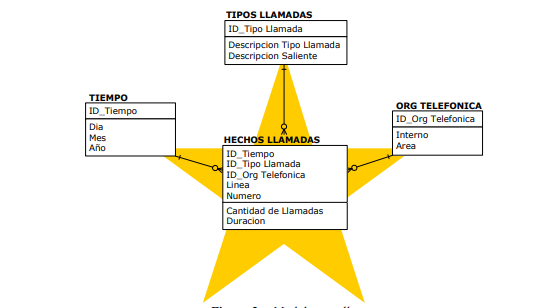
\includegraphics{images/BS/imagen 03.png}\newline
\end{center}

\begin{center}
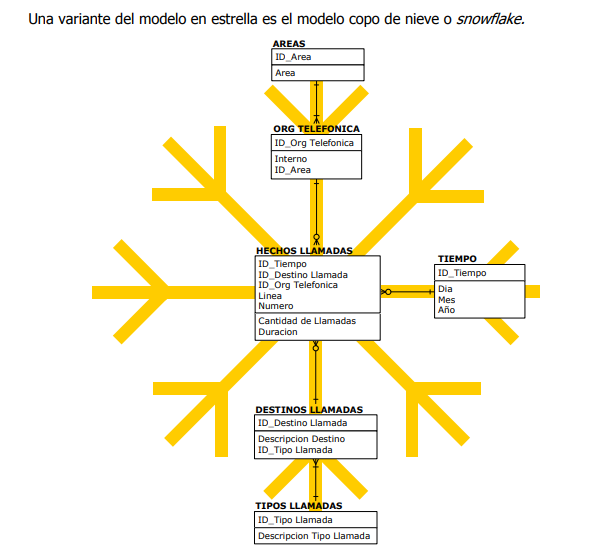
\includegraphics{images/BS/imagen 04.png}\newline
\end{center}



En este modelado se normalizan las dimensiones reflejando las jerarquías en las mismas y conservando lo esencial del modelo en estrella: las tablas de hechos. La ventaja del modelo copo de nieve es eliminar la redundancia de datos y por lo tanto ocupar menos espacio en disco. En la Figura 3 se da un ejemplo de un modelo copo de nieve. \newline 




VENTAJAS DEL MODELO DIMENSIONAL \newline

El modelo dimensional presenta importantes ventajas de las que carece el modelo relacional. Uno de los puntos fuertes del modelo dimensional es que el marco predecible del esquema estrella resiste a los cambios inesperados en el comportamiento del usuario. Cada dimensión es equivalente a las demás y todas las dimensiones pueden ser concebidas como puntos de entrada hacia la tabla de hechos. El diseño lógico puede realizarse independientemente de los patrones de consulta esperados, siendo consideradas de la misma forma tanto las interfaces de usuario como las estrategias de consulta, así como el lenguaje de consulta generado contra el modelo dimensional. \newline 


Otra cualidad del modelo dimensional es la flexibilidad. Los nuevos elementos de datos y las nuevas decisiones de diseño son fácilmente adaptables. Todas las tablas pueden modificarse simplemente agregando nuevos registros de datos o se pueden incluir nuevas dimensiones al modelo sin necesidad de volver a cargar los datos posteriormente. \newline

Además, no es necesario volver a programar las herramientas de consulta o de informes para adaptarse a los cambios, y las aplicaciones existentes pueden continuar su ejecución brindando los mismos resultados. Las modificaciones ante las cuales el modelo dimensional es flexible incluyen: \newline




\begin{itemize}
\item Agregar medidas a la tabla de hechos, siempre que sean aditivas y consistentes con el mayor nivel de detalle de las dimensiones. 
\item Agregar atributos a las dimensiones.  
\item Agregar nuevas dimensiones, siempre que exista un único valor de dicha dimensión definido para cada registro de la tabla de hechos. 
\item Particionar los registros de una dimensión a un mayor nivel de detalle a partir de un determinado punto en el tiempo. Los registros anteriores permanecerán sin cambios mientras que los futuros registros se almacenarán de acuerdo al nuevo modelo. 
\end{itemize}



\subsection{Modelo Tabular}


Los modelos tabulares en Analysis Services son las bases de datos que se ejecutan en memoria o en el modo DirectQuery, conectarse a los datos directamente desde los datos relacionales de back-end orígenes. Mediante el uso de algoritmos de compresión de última generación y el procesador de consultas multiproceso, el motor de análisis de Vertipaq de Analysis Services ofrece un acceso rápido a datos y objetos de modelo tabular mediante la notificación de las aplicaciones cliente como Power BI y Excel. \newline



Aunque los modelos en memoria son el valor predeterminado, DirectQuery es un modo de consulta alternativo para los modelos que son demasiado grandes para caber en memoria, o cuando la volatilidad de los datos impide una estrategia de procesamiento razonable. DirectQuery logra la paridad con modelos en memoria mediante la compatibilidad con una amplia gama de orígenes de datos, capacidad para manejar tablas calculadas y columnas en un modelo DirectQuery, seguridad de nivel de fila a través de expresiones de DAX que llegue a la base de datos back-end y realizar consultas optimizaciones que producen un rendimiento más rápido. \newline


Los modelos tabulares se crean en SQL Server Data Tools (SSDT) mediante la plantilla de proyecto de modelo Tabular. La plantilla de proyecto proporciona una superficie de diseño para crear objetos como tablas, particiones, relaciones, jerarquías, medidas y KPI del modelo semántico. \newline

Los modelos tabulares se pueden implementar en Azure Analysis Services o una instancia de SQL Server Analysis Services configurado para el modo de servidor Tabular. Los modelos tabulares implementados se pueden administrar en SQL Server Management Studio. \newline

Documentación de modelado tabular que se incluyen aquí se aplica en la mayoría de los casos, SQL Server Analysis Services y Azure Analysis Services. \newline


\begin{center}
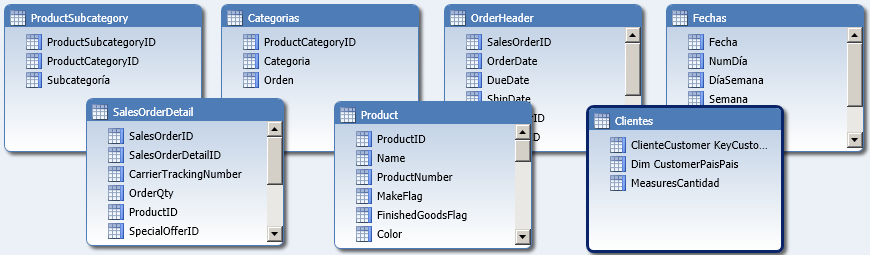
\includegraphics{images/BS/imagen 05.png}\newline
\end{center}


